\chapter{Concept}\label{cha:concept}
\section{Scenario: Mensa Community}
We illustrate the software system by considering a community of frequent canteen visitors. We will call this community the Mensa Community.
The success principle can be applied to this community because community members share a common interest that they are passionate about: the food at their local canteen \cite{Kers20}.
The success factors for this community describe how users are interacting with the service. The members of the Mensa community are students and university employees.

The community has a hierarchical structure consisting of different community levels.
In our case, the top-level represents the community of all canteens in Germany.
The intermediate level represents the local Mensa community of a particular university.
The lowest level of the community represents a circle of friends, which frequent the canteen together. Note that members can belong to multiple circles of friends. Thus communities can be overlapping.

Members of the community use community applications \footnote{\url{https://tech4comp.dbis.rwth-aachen.de/mensa/}}
\footnote{\url{https://monitor.tech4comp.dbis.rwth-aachen.de/}} 
to access information about the Mensa and their community respectively.

Members of the community can interact with a chatbot called \emph{mensabot}. The mensabot is modeled using the Social Bot Framework. 
Users interact with the bot via chat in the Slack workspace of the community. They can ask the bot about the food served on a given day.

As members of the Mensa community are very passionate about the food, they can also use the bot to add a review of their meal.

Furthermore, members can query visualizations about the success of the community through the chat application. Those visualizations include current success metrics defined by members of the community. The metrics are defined using the MobSOS Evaluation Center \cite{Hoss19}. Members can add measures to the success model of the community with the help of the bot.

\subsection{Use Cases}

\subsubsection{Get the menu for the canteen} 
Alice wants to decide whether to go to the canteen on a given day. She opens the Slack app and asks the bot for the menu at the canteen on that day. The bot looks up the menu for that canteen.
The resulting menu is displayed inside the chat. 
Each dish includes an average rating of reviews made by the community. The reviews help Alice decide on a meal.

\subsection{Setting a default city}
Bob asks the bot about the menu for a canteen called \emph{Mensa Academica}. 
The bot finds two canteens matching that name. One is located in Aachen, while the other one is located in Leipzig. 
The bot asks Bob to clarify which canteen he meant by displaying both canteens in a list. Bob chooses the second item in the list. 
The bot returns the resulting menu.
The bot asks him if he wants to save the city, in which his canteen is based as his default city. This helps the bot to identify the canteen on further requests better.

\subsubsection{Adding a review} 
Erdzan just finished his meal at the canteen. To his surprise, the food was better than expected. He decides to do a positive review using the mensabot. 
The bot will start a dialogue by asking questions about the meal. Each question results in a data point for the review. The bot saves the review and displays the result in the chat.

The bot asks him if he wants to upload a photo of his meal. He chooses to do so. The final review is then added to the database and included in future evaluation requests.

\subsubsection{Issuing a visualization request}
Aaron is unsure of whether to go to the canteen. 
He asks the bot how popular a specific canteen is. 
The community had previously defined \emph{popularity} as a measure in the success model. The measure records the number of requests for that canteen's menu and ranks it according to the other canteens.
The bot recognizes this as a predefined measure contained in the success model.
It looks up information about the measure in the measure catalog. 

The measure contains information on how to get the data and how to visualize it. This includes information about the database and the corresponding SQL query on that database. 
The bot transforms this information into a GraphQL request and sends it to the CCA system's GraphQL API. 
The GraphQL server returns the appropriate data.

The bot then visualizes this data and displays the resulting visualization inside the chat.
After the user has seen how good the food is, they are asked by the bot whether they will go to the canteen. They tell the bot that they will go.

\subsubsection{Success Awareness}
Students in the Mensa community are aware that their community's success depends on the active participation of its members. 
They are discussing the success of the community inside a group chat. They want to know how active the members of the community are. One student calls the bot, which is a member of the chat group, by name. They tell it to visualize the average time that a user is interacting with the service. The bot recognizes this as a measure and runs a predefined query. The resulting data is visualized in the group chat.

\subsubsection{Success modeling} 
The students see a trend in the visualization, which indicates that fewer people are using the bot.
The students blame the Coronavirus for this negative trend as the canteen can only be used as takeout. Furthermore, many students returned to their hometowns.
The students want to verify that the lack of activities is due to the Coronavirus and not decreasing food quality.
They ask the bot to update the success model of their community.
They add a measure that models the average stars of reviews over time.
After visualizing the new metric, they observe that the average stars have remained more or less constant over time.

The students are asked to add a comment to the change so that community members can understand the reason for the change at a later date.


\subsubsection{Modifying a review} 
Alexander just added a review to the database. He realizes that he forgot to mention the excellent quality of the fries. 
He asks the bot if he can still update his review. 
The bot will ask the user the same questions and, afterward, update the entry in the new review database.

\subsubsection{Evaluating the service} 
Peter has been using the bot for some time now. The bot asks questions about the quality of the service. Such questions include how satisfied he is with different aspects of the service or how likely it is to recommend it to a colleague. The results are used for measures in the User Satisfaction dimension.

\subsubsection{Adding a new database} 
Core members and moderators of the community can add a new information source by adding a new database to the system. They do it using the frontend of the CCA service and the MobSOS query visualization service.
The moderators are aware that many members of the community also add reviews on sites like Google reviews. 
They add a Mediabase containing reviews collected by crawlers from sites like Google Reviews. Those reviews can now also be used for success modeling.

\subsubsection{Visualizations of multiple databases} 
Multiple databases can exist in a system. Apart from the reviews added by chat, other reviews are also collected with crawlers. A student requests a visualization of a metric that represents the overall success of the community.
The data is aggregated from different sources, like reviews on Facebook, Google, stored in the Mediabase, and reviews made inside the las2peer system. 
The resulting visualization contains all databases' results to define how popular the specific canteen is.

\begin{figure}
    \centering
    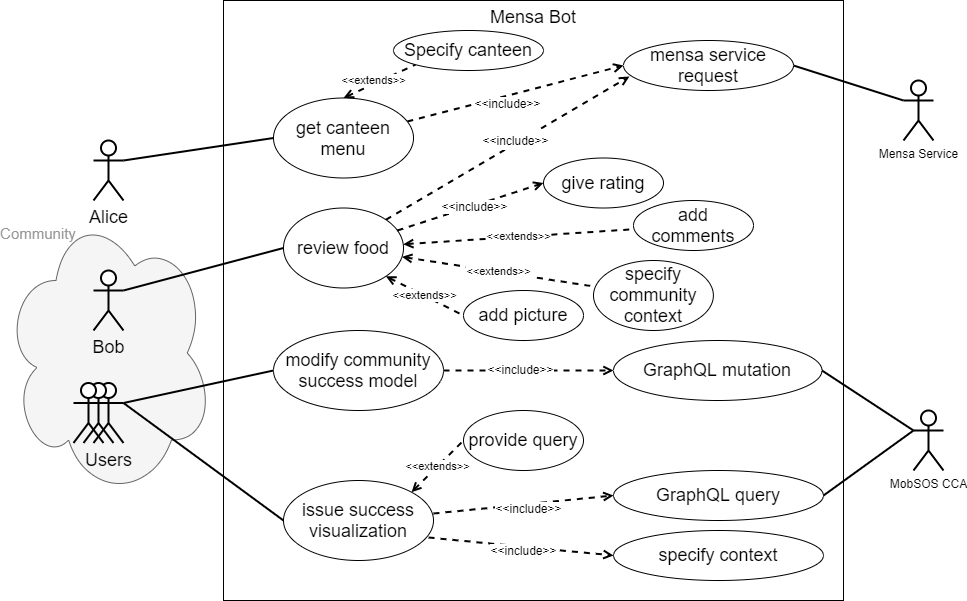
\includegraphics[width=0.8\linewidth]{concept/usecase.png}
    \caption{Use case diagram for the Chatbot}
\end{figure}

\section{Requirements}
The requirements are derived from the use case. We distinguish between functional and non-functional requirements.
\subsection{Functional Requirements}

\subsubsection{Retrieving Data from GraphQL API}
The system needs to be able to make queries to the GraphQL API, to get data, which will be used to visualize success metrics. The GraphQL API  for the Continuous Community Analytics systems provides data from different data sources, such as a las2peer database, a Mediabase with data collected from outside the las2peer system, and a database contains service logs.

\subsubsection{Get Menu for a canteen} The bot needs to be able to get the menu for a specific canteen for the given day and display it inside the chat as a list of text items. The service should be able to use the OpenMensa API \footnotemark to get the menu for canteens all over Germany.

\footnotetext{\href{https://doc.openmensa.org/api/v2/}{https://doc.openmensa.org/api/v2/}}

\subsubsection{Enter Review Context} The bot should be able to recognize if a user wants to start a review. This can be done with the help of intent recognition from a RASA server.

\subsubsection{Group Chats} Users should be able to add a bot to a group chat.

\subsubsection{Listen to Mentions} Inside a group chat, the bot should only respond to messages which specifically mentioned the bot. This is important to prevent the bot from spamming the chat.

% \subsubsection{Create new templates} The bot needs to be able to create visualization-request templates and add them to the database.

\subsubsection{Use Google Charts API}
The data retrieved from the GraphQL API needs to be passed to the Google Charts API to create a visualization. The resulting visualization should be a picture so that it can be represented inside a chat. The visualization can be rendered by using an HTML image generator.

\subsubsection{Cope with spelling mistakes} The bot should be able to understand the user, even if they made a spelling mistake.

\subsection{Non-Functional Requirements}

\subsubsection{Usability} The bot should be easy to use. Non-trained users should be able to interact with the bot with ease.

\subsubsection{UI optimization} The bot should be designed for chats which will mainly run on smartphones. As such, visualizations should be easy to read, even on small devices.

\subsubsection{Compatibility} The bot should be extensible to any chat platform, which allows the use of bots.

\section{System overview}


\begin{figure}[h]
    \centering
    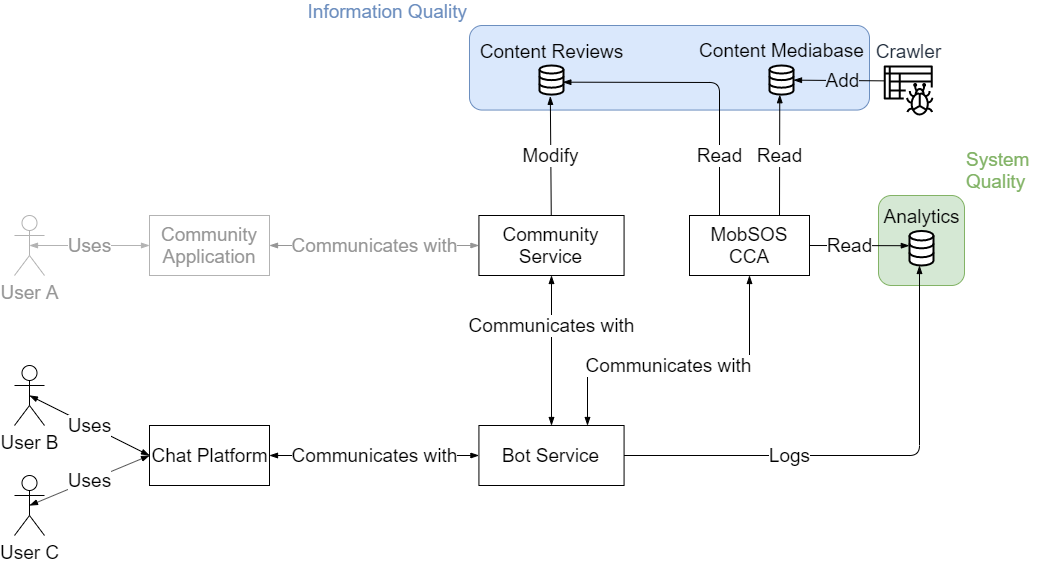
\includegraphics[width=\linewidth]{realization/Component_Diagramm.png}
    \caption{System overview}
    \label{fig:sytsemOverview}
\end{figure}

Figure \ref{fig:sytsemOverview} shows how the \emph{Bot Service} can be integrated into an existing community information system. Users communicate with the \emph{Chat Platform}, which transmits requests to the Bot Service.

The Bot Service communicates with the \emph{Community Service} to provide users the same, or similar, information as an existing \emph{Community Application}. The bot service also communicates with the \emph{MobSOS CCA} system to retrieve success visualizations and display them as charts on the Chat Platform. Users can also use the chat to model success queries and modify the existing success model.

Both the community service and the bot service generate logs from requests. The logs are stored in a database representing the \emph{System Quality} dimension of the MobSOS success model. The MobSOS CCA system can retrieve those logs. Furthermore, the MobSOS CCA system also has access to various content databases that represent the \emph{Information Quality} dimension of the MobSOS success model.